\let\negmedspace\undefined
\let\negthickspace\undefined
\documentclass[journal]{IEEEtran}
\usepackage[a5paper, margin=10mm, onecolumn]{geometry}
%\usepackage{lmodern} % Ensure lmodern is loaded for pdflatex
\usepackage{tfrupee} % Include tfrupee package

\setlength{\headheight}{1cm} % Set the height of the header box
\setlength{\headsep}{0mm}  % Set the distance between the header box and the top of the text

\usepackage{gvv-book}
\usepackage{gvv}
\usepackage{cite}
\usepackage{amsmath,amssymb,amsfonts,amsthm}
\usepackage{algorithmic}
\usepackage{graphicx}
\usepackage{textcomp}
\usepackage{xcolor}
\usepackage{txfonts}
\usepackage{listings}
\usepackage{enumitem}
\usepackage{mathtools}
\usepackage{gensymb}
\usepackage{comment}
\usepackage[breaklinks=true]{hyperref}
\usepackage{tkz-euclide} 
\usepackage{listings}
% \usepackage{gvv}                                        
\def\inputGnumericTable{}                                 
\usepackage[latin1]{inputenc}                                
\usepackage{color}                                            
\usepackage{array}                                            
\usepackage{longtable}                                       
\usepackage{calc}                                             
\usepackage{multirow}                                         
\usepackage{hhline}                                           
\usepackage{ifthen}                                           
\usepackage{lscape}

% Marks the beginning of the document
\begin{document} 
\bibliographystyle{IEEEtran}
\vspace{3cm}

\title{4-4.2-5}
\author{EE24BTECH11029- JANAGANI SHRETHAN REDDY}
\maketitle
\bigskip
\renewcommand{\thefigure}{\theenumi}
\renewcommand{\thetable}{\theenumi}
\textbf{Question:}
Find the direction and normal vectors of the line $2x=-5y$.\\
\solution\\

direction vector$=m$\\
normal vector$=n$\\
\begin{align}
\frac{x}{-5}&=\frac{y}{2}\\
 m&=\myvec{-5\\2}\\
 n&=\myvec{2\\5}
\end{align}
 \begin{figure}[h!]
  \centering
  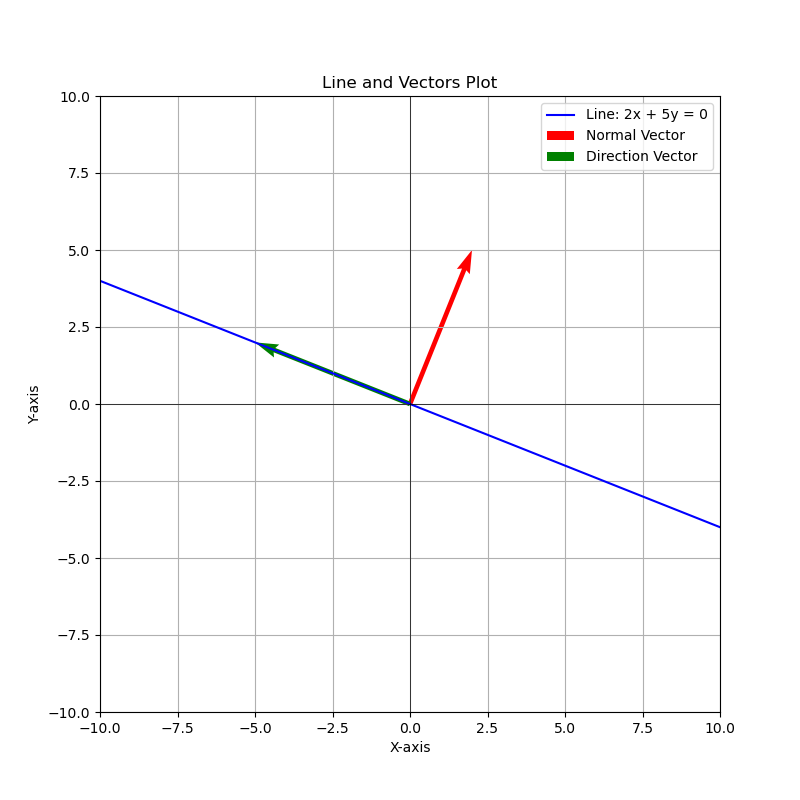
\includegraphics[width=1\linewidth]{fig/fig.png}
  \caption{plot of m and n}
 \end{figure}
\end{document}

